\documentclass[a4paper,UTF8]{ctexart}

\usepackage{float}
\usepackage{hyperref}
\usepackage{setspace}
\usepackage{indentfirst} % 首行缩进

% 正文格式设置
\setlength{\parindent}{2em}     % 首行缩进 2 个字符

\renewcommand\normalsize{
    \zihao{5}\songti
    \linespread{1.25}\selectfont
}

% -------- 层级标题格式 --------
% 第一层:一、二、三……
\ctexset{
  section = {
    format = \zihao{5}\heiti\bfseries, % 五号 黑体 加粗
    name = {,、},                      % “一、”
    number = \chinese{section}         % 中文数字
  },
  % 第二层:(一)(二)(三)……
  subsection = {
    format = \zihao{5}\kaishu,         % 五号 楷体
    name = {(,)},                      % 括号
    number = \chinese{subsection}
  },
  % 第三层:1. 2. 3. ……
  subsubsection = {
    format = \zihao{5}\songti,         % 五号 宋体
    name = {},                         % 去掉默认小标题文字
    number = \arabic{subsubsection}.   % 阿拉伯数字加点
  }
}

% 行距
\usepackage{setspace}
\onehalfspacing
% 图表支持
\usepackage{graphicx}
\usepackage{caption}
\usepackage{subcaption}
\usepackage{array}
\usepackage{booktabs}

% 页眉页脚 页面设置
\usepackage{fancyhdr}
\usepackage[top=3cm,bottom=3cm,left=2.6cm,right=2.6cm]{geometry}
\setlength{\headheight}{14pt}
\setlength{\headsep}{10pt}
\pagestyle{fancy}
\fancyhf{}
\fancyhead[C]{人工智能工程实践project报告}
\fancyfoot[C]{\thepage}


\begin{document}
\begin{center}
\vspace*{1cm}
{\heiti \bfseries \zihao{2} “知食”饮食助手AI Agent项目报告 \par}
\vspace{1cm}
{\kaishu \zihao{5} 第9组成员:陈丽珊、何欣艺、黄乐隽、汪晨恺 \par}
\end{center}

{\bfseries 小组分工:}
\begin{center} 
\begin{tabular}{|l|l|l|l|}
\hline
\textbf{姓名} & \textbf{学号} & \textbf{专业} & \textbf{任务分工} \\ \hline
陈丽珊 & 3240105497  & 人工智能 & 工作流、智能体搭建;PPT、报告撰写与完善\\ \hline
何欣艺 & 3240102760 & 信息工程 & 网页开发;工作流搭建; PPT、报告撰写与完善\\ \hline
黄乐隽 & 3240100711 & 人工智能 & PPT、报告撰写 \\ \hline
汪晨恺 & 3240100428 & 人工智能 & PPT、报告撰写 \\ \hline

\end{tabular}
\end{center}


\section{项目背景}
实际生活需要:随着社会发展和生活水平提高,人们对健康生活
的追求日益增长。科学饮食作为健康管理的核心环节,受到广泛关注。
然而,普通用户在面对“减脂期该吃什么?”、“健身前后如何补充
营养?”、“这份食物的热量是多少?”、“附近有哪些健康餐厅?”
等问题时,往往缺乏专业、便捷的获取答案的渠道。传统的信息检索
方式耗时耗力,且信息质量良莠不齐。
\par
模型优势:大型语言模型(LLM)在自然语言理解和生成方面展
现出强大能力,为本问题提供了全新的解决方案。通过将LLM的通
用知识与专业的营养学数据库、地理位置服务(如高德地图API)相
结合,我们可以构建一个智能、交互式的专业营养膳食助手Agent,
为用户提供即时、精准、个性化的膳食建议。

\section{项目目标}
本项目旨在设计并实现一款基于百炼平台的人工智能 Agent 应用——“营养膳食助手”。该 Agent 应能通过自然对话的方式,理解用户的膳食需求,并调用相应的工具API为用户提供专业服务。具体实
现以下四个核心功能:
\subsection{食物营养成分查询}
快速查询特定食物的详细营养成分数据,包括热量、蛋白质、脂肪、碳水化合物、维生素等。
\subsection{菜谱生成}
根据食材、菜品名等信息生成合理、详细、健康的菜谱。
\subsection{个性化饮食推荐}
根据用户的目标(如减脂、增肌、维持健康)和自身身体状况,自身偏好等条件,推荐科学合理的每日或单餐食谱。
\subsection{餐厅推荐与路径规划}
基于用户所在或指定的地区,以及用户的要求和条件,推荐符合健康膳食标准的餐厅。若用户有需要,小助手可以为用户进行路径规划。


\section{技术实现}
\subsection{核心工具}
\subsubsection{阿里百炼平台}
我们本次设计通过阿里云百炼平台进行,其核心优势在于可视化的工作流编排能力,允许我们以低代码的方式,将大模型、API调用、条件判断、代码脚本等功能模块像积木一样搭建和连接。这不仅极大地提升了开发效率和调试速度,也使得复杂的 Agent 内部逻辑变得清晰、可管理。同时,依托于阿里平台丰富的应用生态,百炼提供了许多功能丰富、开箱即用的工具,为我们的功能实现提供了很大的便利,我们本次使用了路径规划、高德地图和今天吃什么 MCP 辅助我们的智能体开发。
\subsubsection{通义千问大模型}
我们选用通义千问大模型作为本次智能体开发的基础。该模型是阿里巴巴集团自主研发的大语言模型体系,具备强大的理解、生成与处理自然语言和代码的能力,在多项权威评测和实际应用中表现出卓越的性能。通义千问支持超长上下文推理,可处理长达数百万token的文本,进行高效分析与内容生成。
\subsubsection{外部 API}
Spoonacular 是一个功能极其强大的食品、营养和食谱数据 API,为开发者、营养师、食品博主、健身应用和任何对食品数据感兴趣的人提供了一个庞大的数据库和一系列工具。其拥有一个包含超过 36 万份食谱的庞大数据库,每份食谱均配有标题、图片、食材清单、具体用量、烹饪步骤、准备时间、难度等级及详细营养成分等完整信息。其先进的智能搜索不仅支持按菜名查询,还能根据用户现有食材进行个性化推荐,同时提供精细的高级过滤功能,可依据饮食要求、菜系风味、过敏原限制及营养成分需求进行多维度筛选。系统还集成了涵盖数千种食材的详细营养数据库(包括热量、蛋白质、脂肪、碳水化合物、维生素和矿物质等),支持对任意食谱或组合餐品进行总营养含量计算。

\subsection{实现过程}
\subsubsection{大体框架}
我们构建了一个“总指挥智能体 + 多个专业工作流”的协同任务处理体系。在这个体系中,顶层智能体作为统一入口,负责接收用户请求、理解真实意图,并进行智能任务规划与任务分发;而各项专业任务则由对应的专项工作流精细处理,包括调用本地餐厅推荐(集成高德地图API)、生成个性化菜谱(通过“今天吃什么”MCP)、查询营养成分(接入Spoonacular API)以及进行路径规划(使用路径规划MCP)等。每个工作流职责清晰、功能专注,既可独立优化也可灵活复用,最终通过统一的前端渠道(网页和微信公众号)为用户提供便捷高效的服务体验。
\begin{figure}[H]
    \centering
    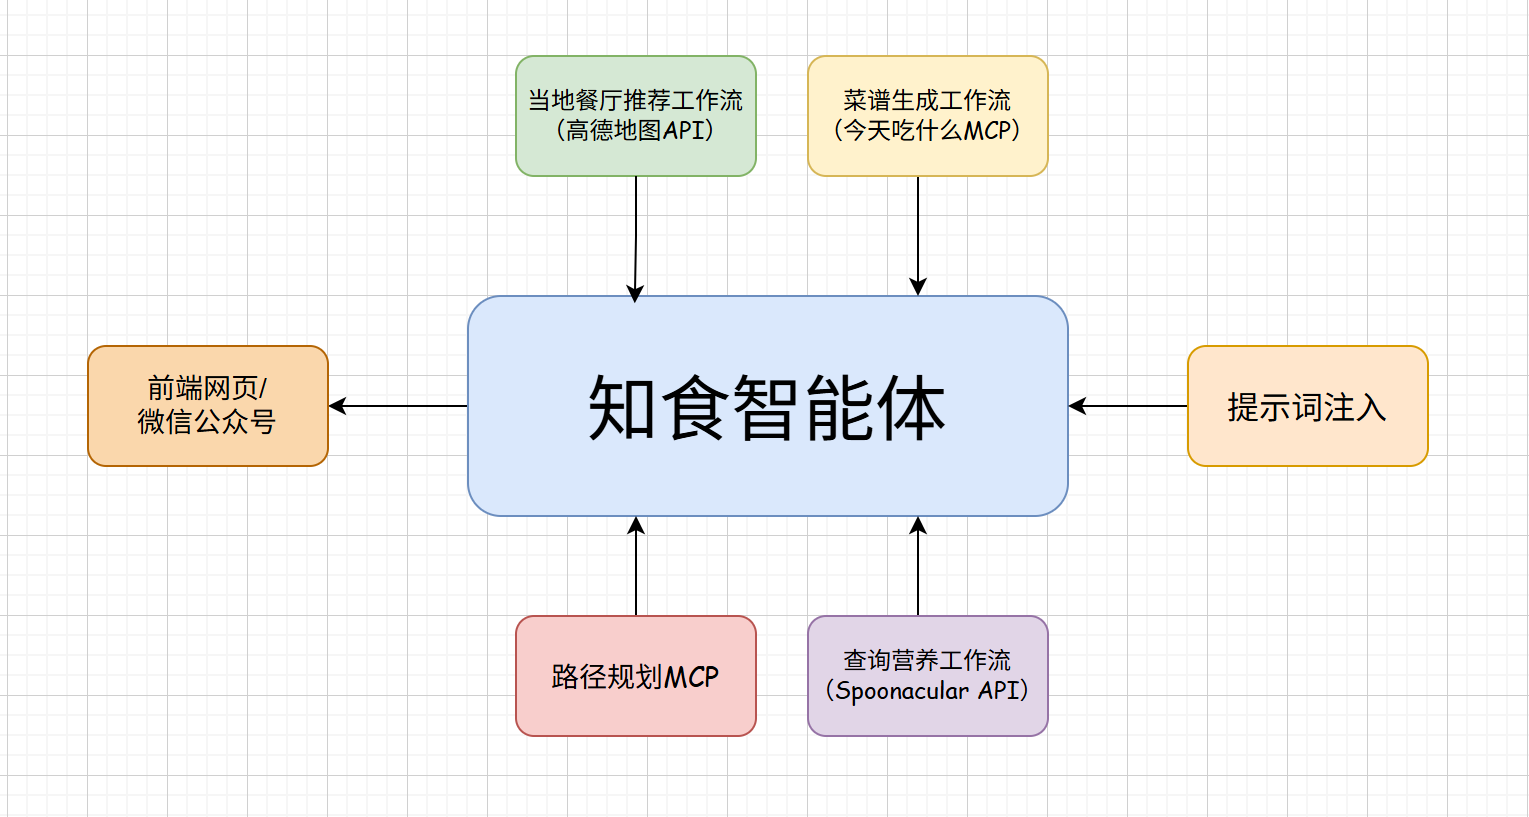
\includegraphics[width=0.8\linewidth]{0.png}
    \caption{大体框架}
    \label{fig:diet_recommend}
\end{figure}

\subsubsection{提示词设置}

{\bfseries 智能体层提示词:}通过提示词注入赋予顶层智能体“知食”的完整的角色设置和人格品质,如“你的最高使命是:通过科学、个性化且充满乐趣的饮食指导,赋能用户建立与食物之间更健康、更愉悦的关系”“共情: 你能理解用户在饮食管理中可能遇到的困惑、挫败感和喜悦;耐心: 你从不厌烦用户的重复提问或初步的知识盲点;风趣: 在保持专业的同时,你的语言风格带有一丝轻快的风趣”;规定其回答的边界,如“对医疗相关问题,须建议用户咨询专业人士”,以保证用户的健康与安全;
为其设定了清晰的决策框架,智能判断用户的请求是否与所接入的工作流功能相关,如果是则根据具体情况调用工作流,反之则基于自身角色设置回答用户的问题,并引导用户提问与“知食”智能体核心功能相关的问题。
\par
{\bfseries 工作流层提示词:}在工作流内部,我们为不同的大模型节点设计了高度功能化的提示词。例如,“参数提取”节点的提示词包含了多个示例,严格规定了输出的 JSON 格式和每个字段的提取规则,确保了结构化数据的稳定输出。而“结果输出”节点的提示词则侧重于风格转换和数据总结,确保了智能体输出的最终质量,提高用户体验感。

\subsubsection{工作流搭建}
{\bfseries 查询营养工作流:}
\begin{figure}[H]
    \centering
    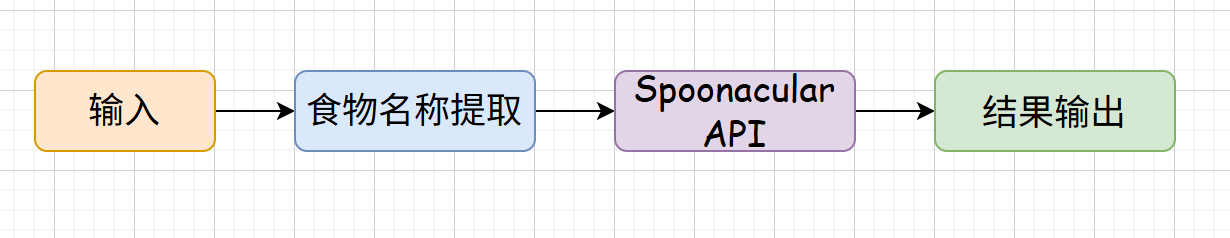
\includegraphics[width=0.8\linewidth]{0-1.png}
    \caption{查询营养工作流}
    \label{fig:diet_recommend}
\end{figure}

{\bfseries 菜谱生成工作流:}
\begin{figure}[H]
    \centering
    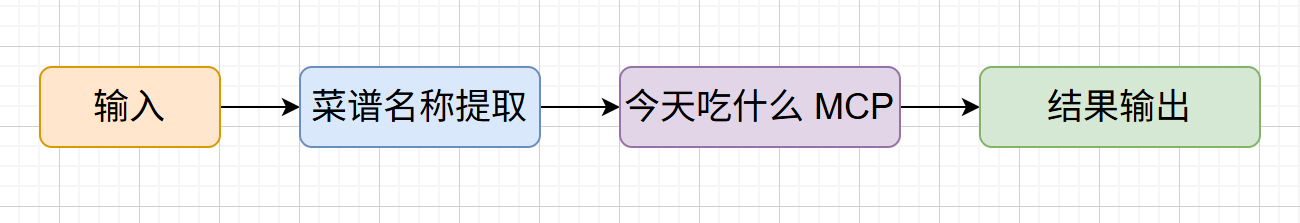
\includegraphics[width=0.8\linewidth]{0-2.png}
    \caption{菜谱生成工作流}
    \label{fig:diet_recommend}
\end{figure}

{\bfseries 餐厅推荐工作流:}
\begin{figure}[H]
    \centering
    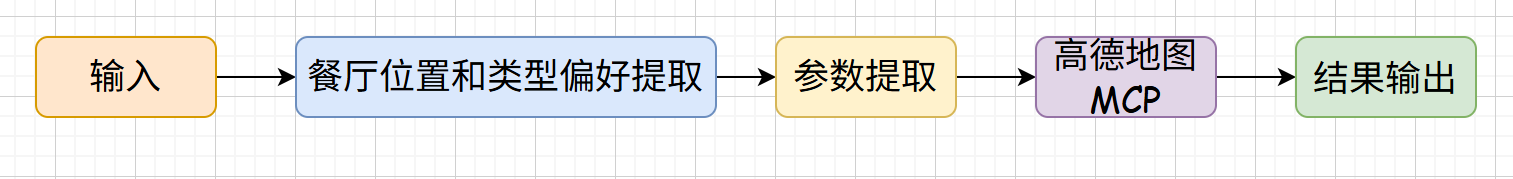
\includegraphics[width=0.8\linewidth]{0-3.png}
    \caption{餐厅推荐工作流}
    \label{fig:diet_recommend}
\end{figure}

\subsubsection{前端实现}
基于Python。
\par
代码详情可见于我的gitee仓库:\url{https://gitee.com/wander20250901/ai_-agent_diet.git} $->$ main分支 $->$ project
\begin{figure}[H]
    \centering
    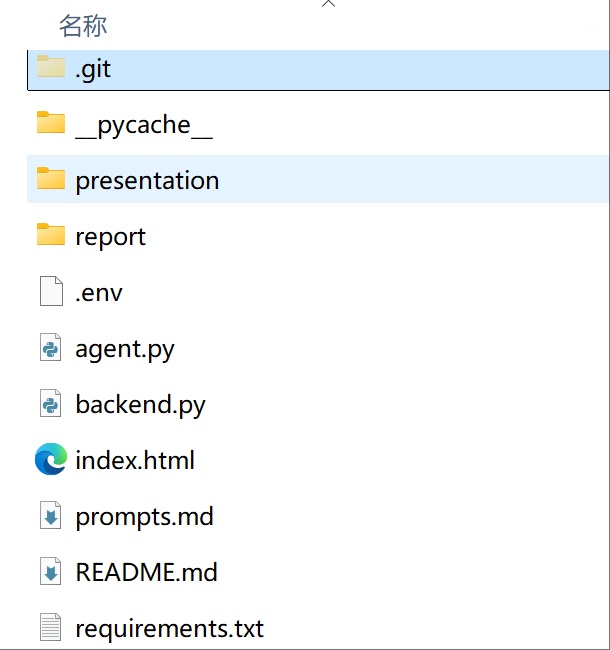
\includegraphics[width=0.55\linewidth, height=6.5cm]{5-1.png}
    \caption{网页开发文件夹}
    \label{fig:diet_recommend}
\end{figure}

\subsubsection{pre后的优化}
相较于在课堂展示中所呈现的单一工作流,我们通过将其拆分为不同功能模块的多条工作流,并进一步修改优化提示词,让大语言模型可以根据用户输入的具体情况,智能选择调用工作流,实现了在一次交互中调用多个不同工作流和调用同一功能工作流多次,使得不同分支工作流之间可以联动使用,提高其智能性,简单的闲聊则由顶层智能体直接处理,避免了不必要的资源消耗,提高了运行效率,综合提升用户体验。并且,每个专业工作流都是一个高度优化、职责单一的模块,内部封装了从参数提取、API调用到结果处理等完整的多步逻辑,各功能模块相互独立,调试和优化更为精准,未来新增功能只需增加新的工作流,而无需改动整体框架,极大地提升了系统的可维护性和可扩展性。


\section{最终效果}
\subsection{查询食物营养信息}
\begin{figure}[H] 
  \centering 
  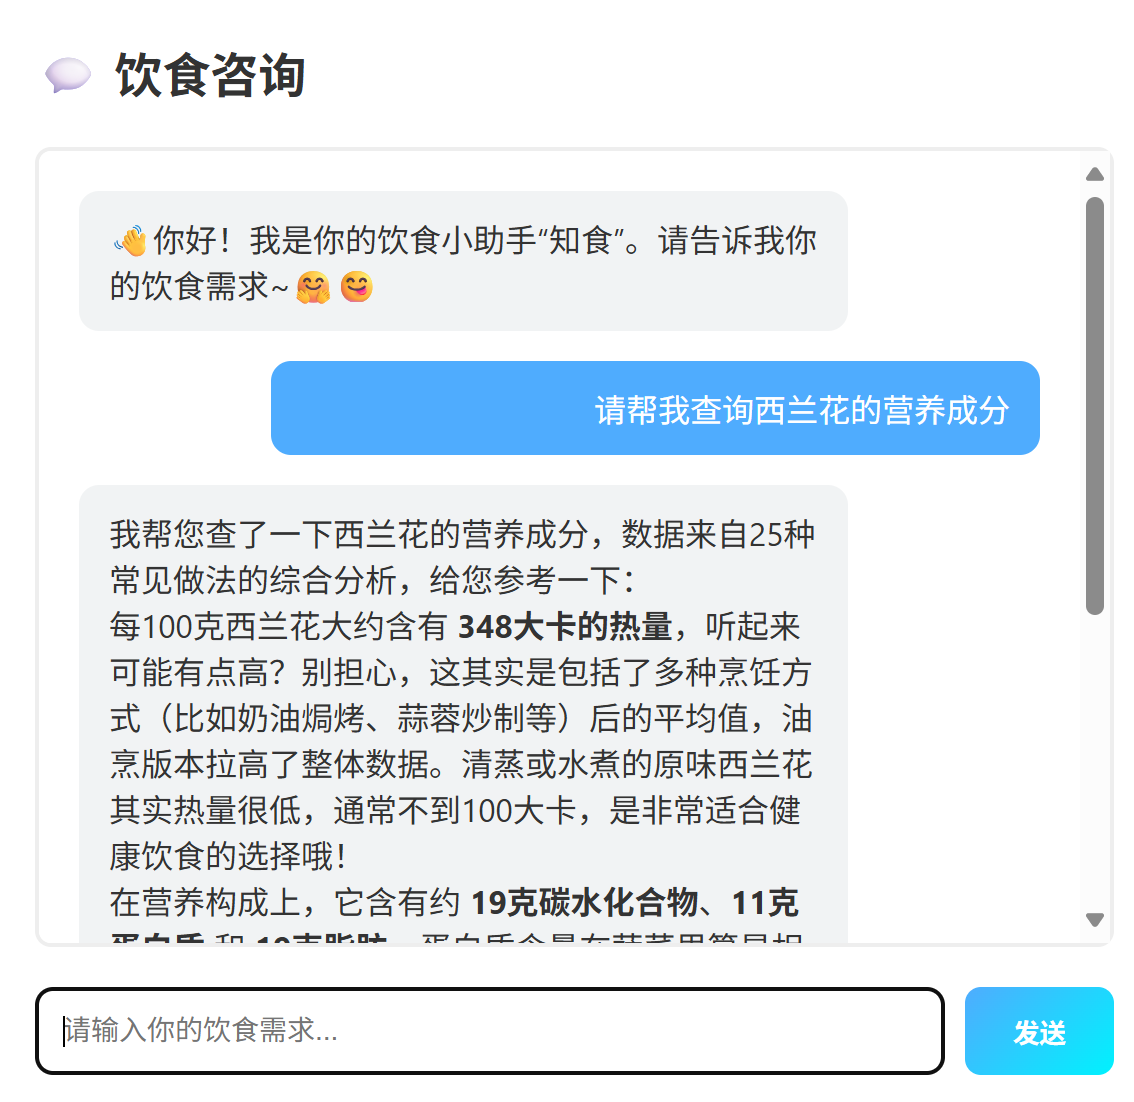
\includegraphics[width=0.8\linewidth,height=0.42\textheight,keepaspectratio]{1-1.png}\\[1ex] 
  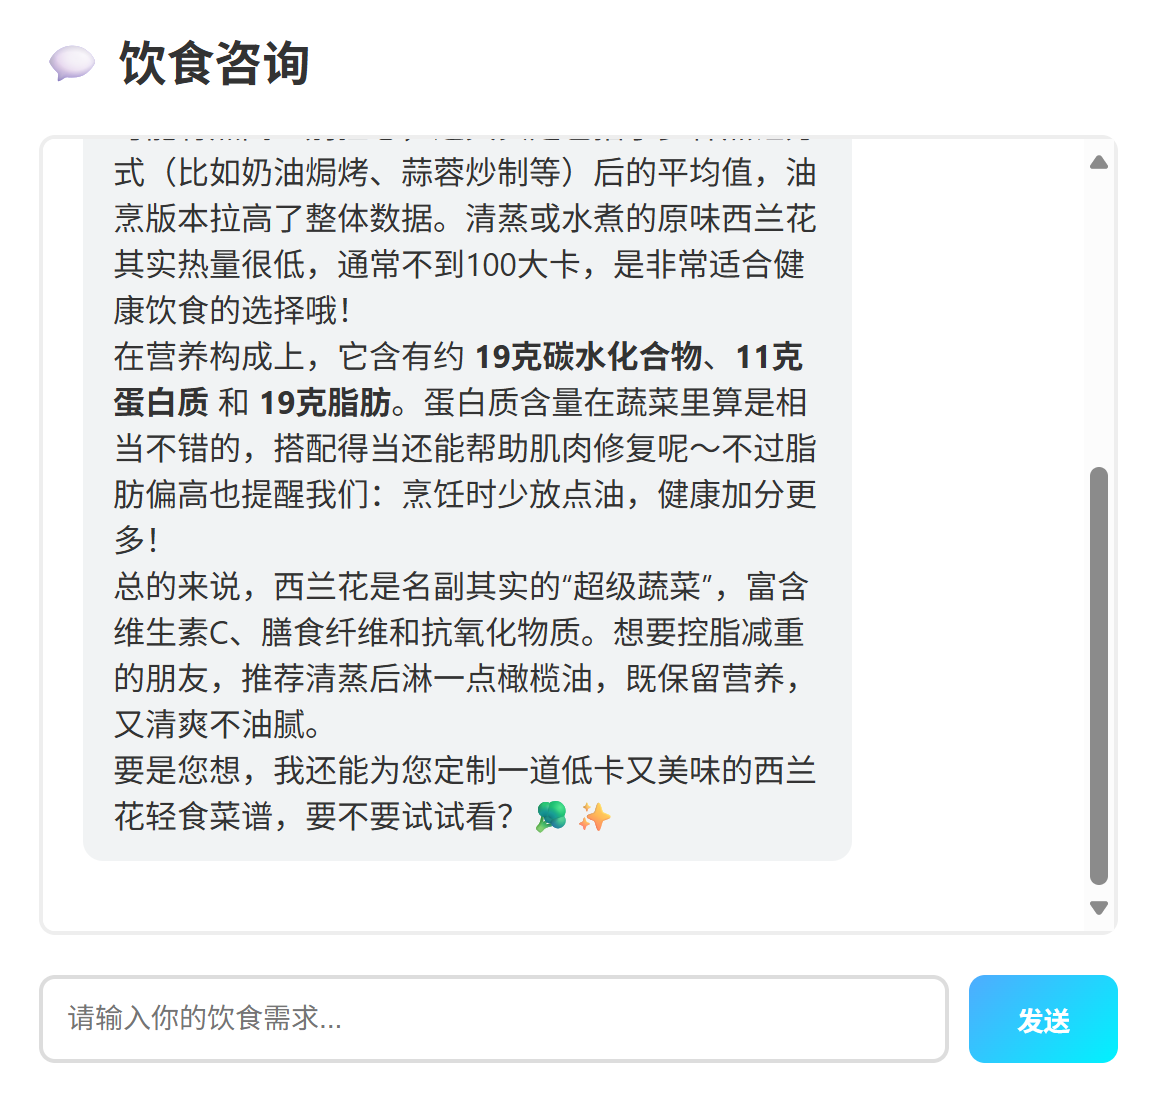
\includegraphics[width=0.8\linewidth,height=0.42\textheight,keepaspectratio]{1-2.png}\\[1ex] 
  \caption{查询食物营养信息} 
  \label{fig:diet_recommend} 
\end{figure}

\subsection{生成菜谱}
\begin{figure}[H]
    \centering
    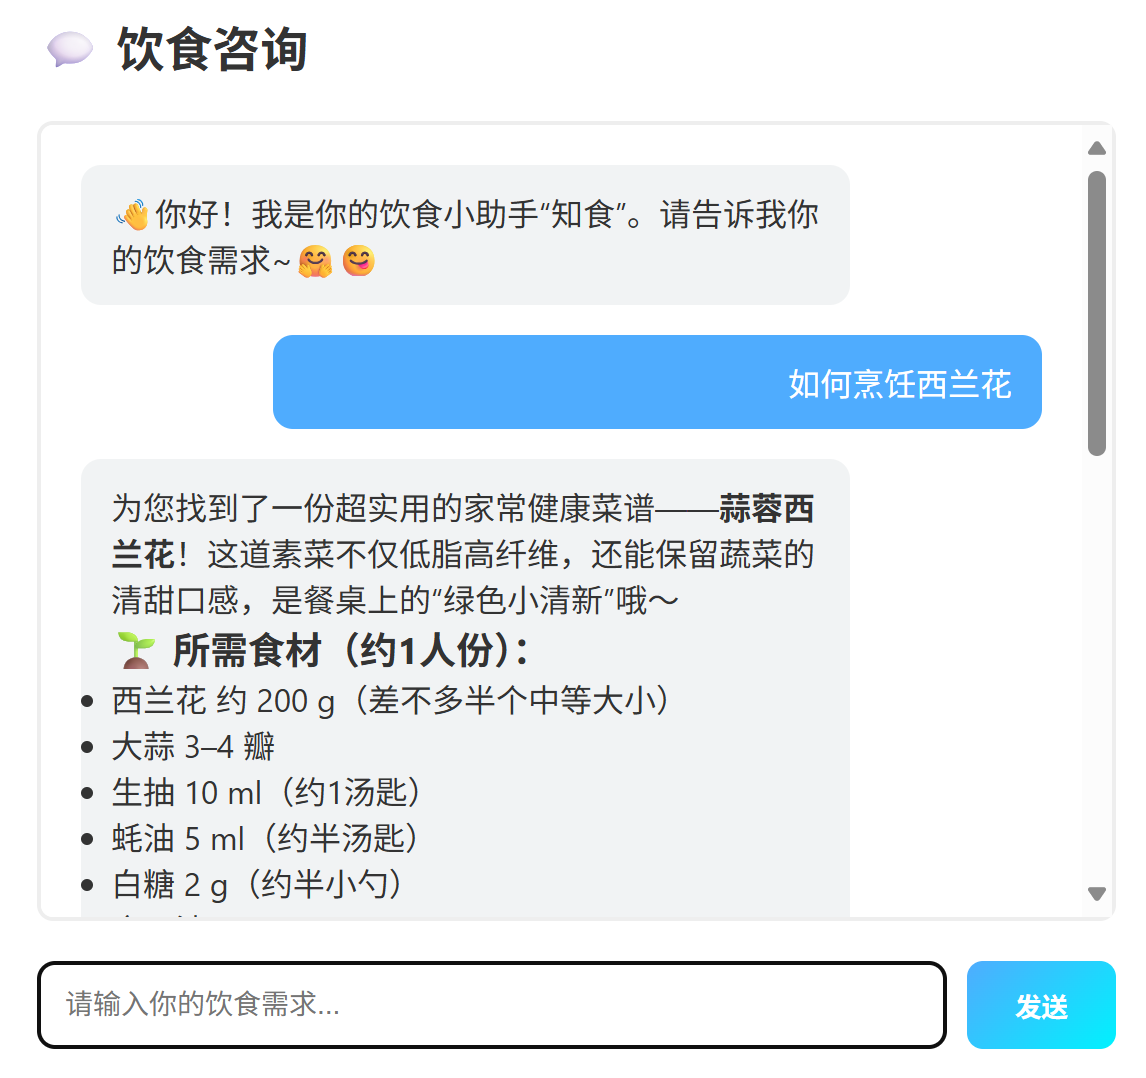
\includegraphics[width=0.8\linewidth,height=0.45\textheight,keepaspectratio]{2-1.png}\\[1ex]
    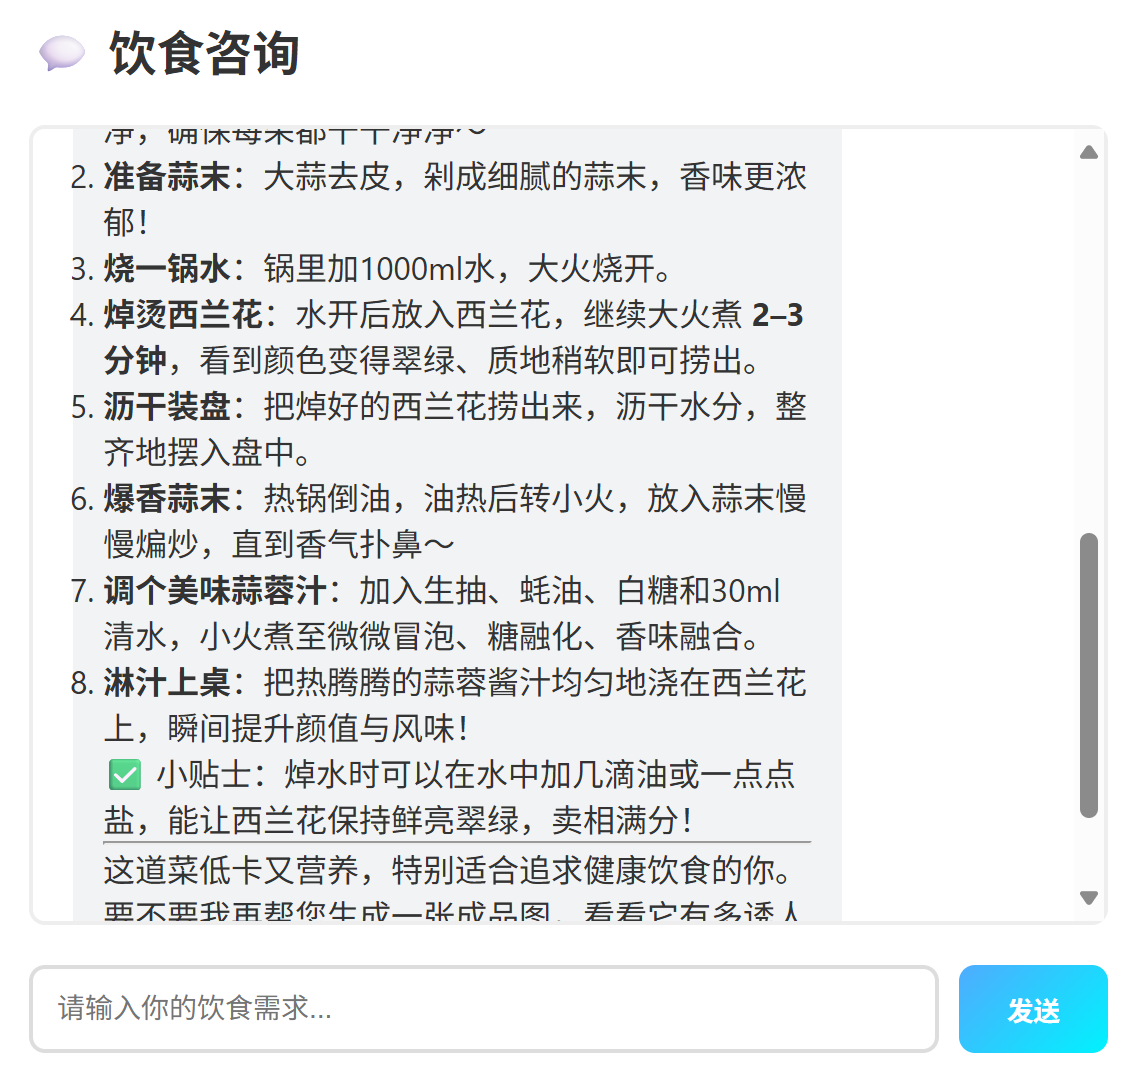
\includegraphics[width=0.8\linewidth,height=0.45\textheight,keepaspectratio]{2-2.png}\\[1ex]
    \caption{生成菜谱}
    \label{fig:diet_recommend}
\end{figure}

\subsection{个性化饮食推荐}
\begin{figure}[H]
    \centering
    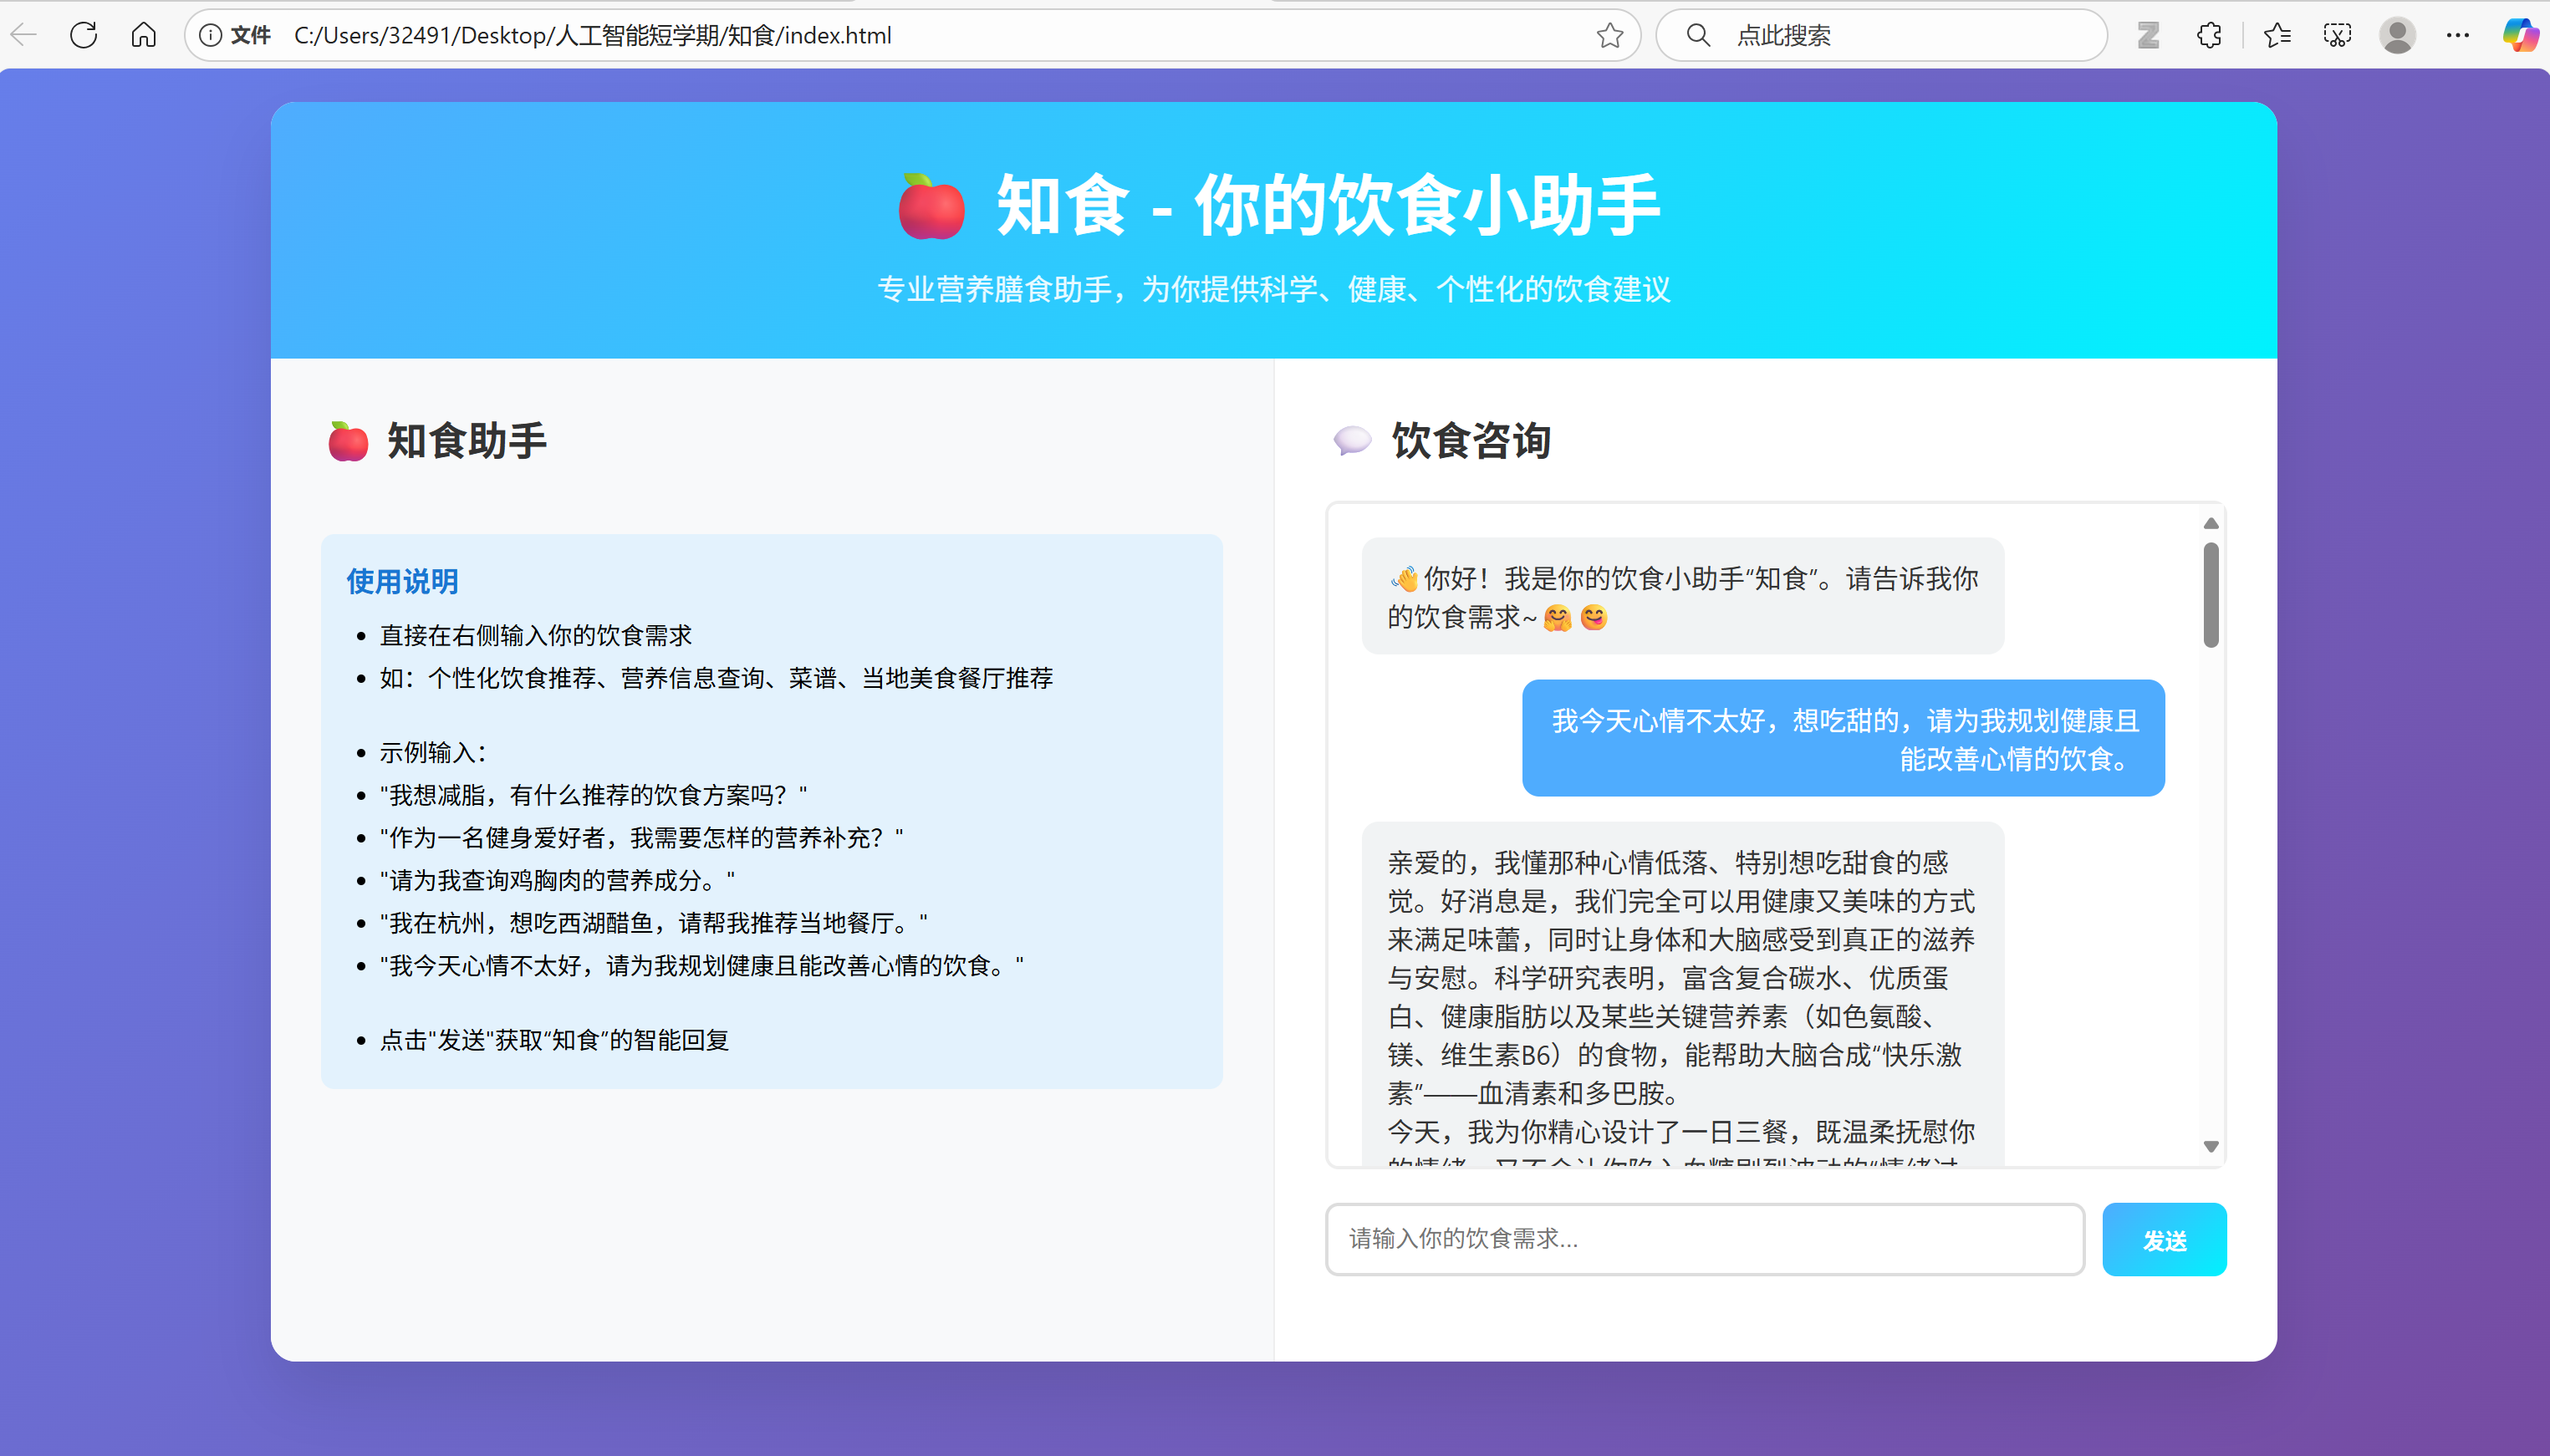
\includegraphics[width=0.8\linewidth,height=0.3\textheight,keepaspectratio]{1.png}\\[1ex]
    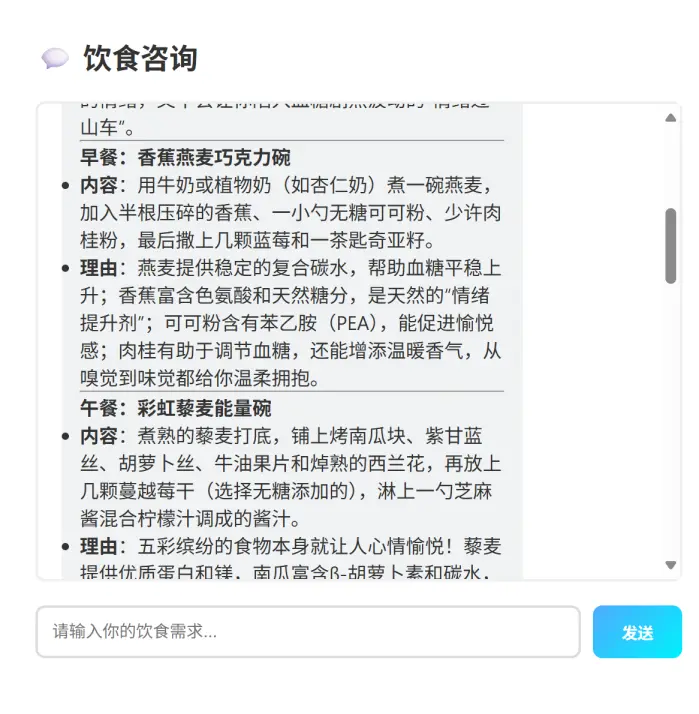
\includegraphics[width=0.8\linewidth,height=0.3\textheight,keepaspectratio]{2.png}\\[1ex]
    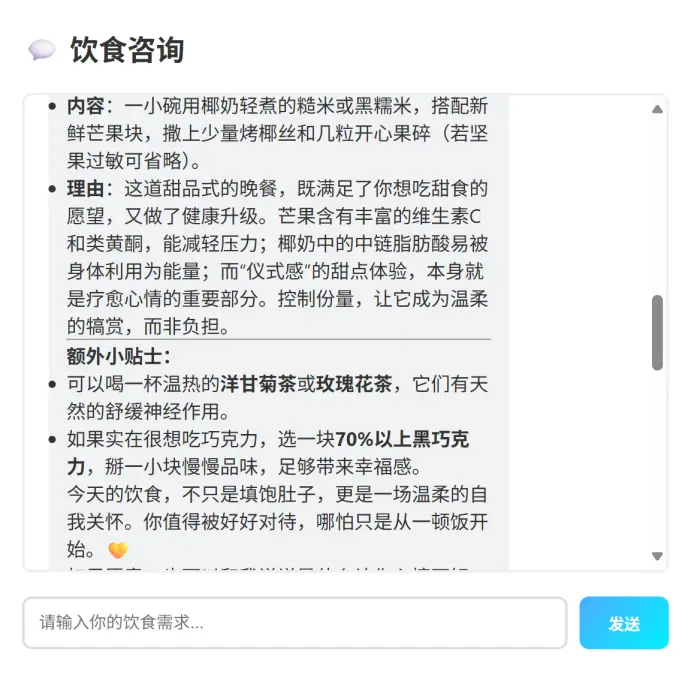
\includegraphics[width=0.8\linewidth,height=0.3\textheight,keepaspectratio]{3.png}
    \caption{个性化饮食推荐}
    \label{fig:diet_recommend}
\end{figure}

\subsection{餐厅推荐}
\begin{figure}[H]
    \centering
    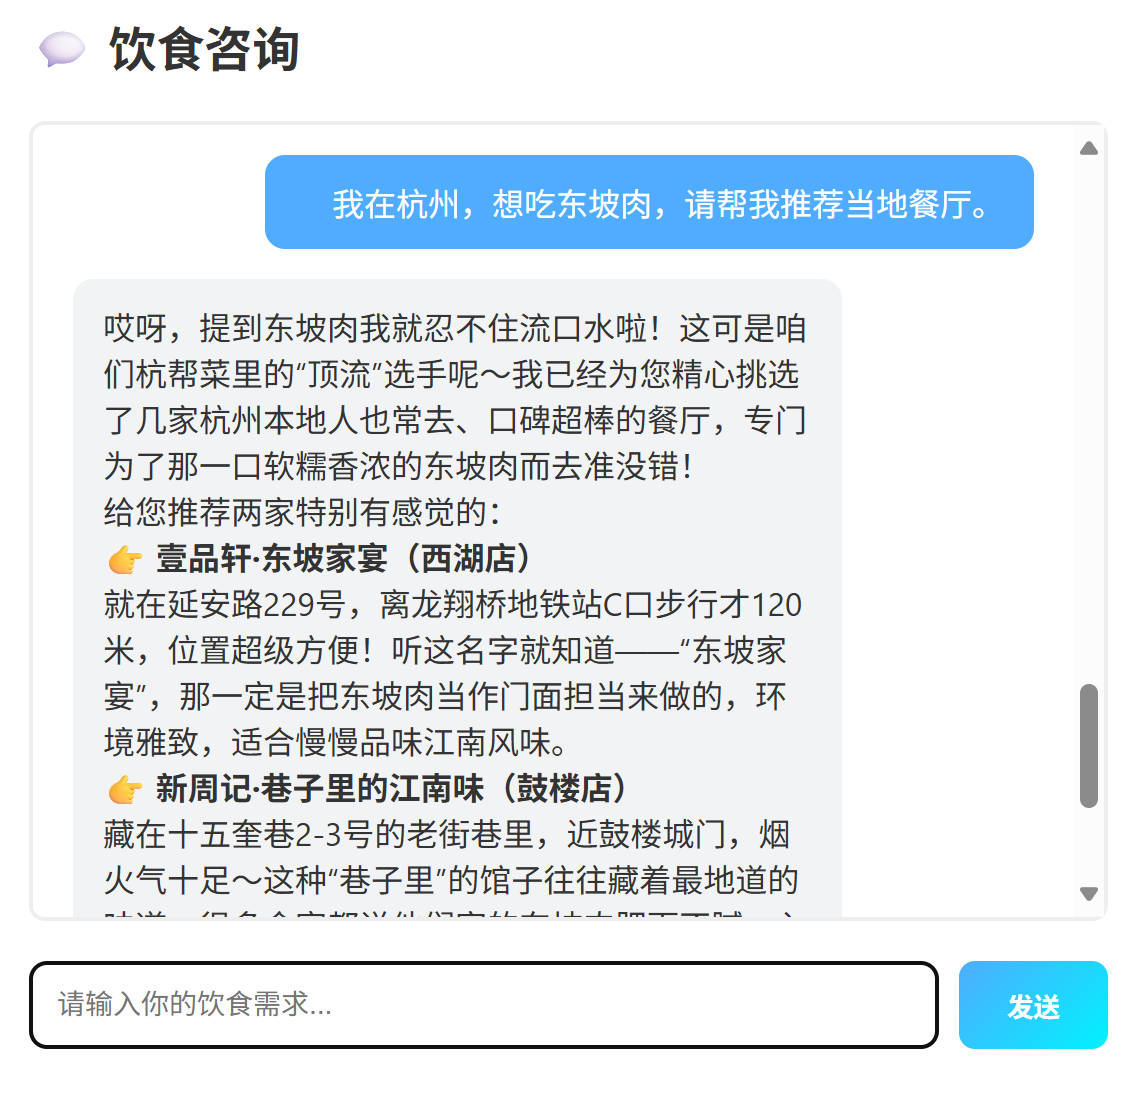
\includegraphics[width=0.8\linewidth,height=0.4\textheight,keepaspectratio]{4.png}
    \caption{餐厅推荐}
    \label{fig:diet_recommend}
\end{figure}

\section{总结与展望}
本次项目围绕“知食”饮食助手的设计与实现展开,团队从背景问题出发,提出了个性化饮食推荐的整体方案。通过引入通义千问大模型和阿里百炼平台,结合外部 API(如 Spoonacular、地图服务等),我们实现了营养信息查询、菜谱生成等核心功能,并初步探索了餐厅推荐与个性化饮食规划的方向。
\par
在项目实施过程中,我们经历了从基础功能搭建到逐步完善的过程,积累了在大模型应用、API 调用和工作流设计方面的实践经验。尽管目前仍存在语义理解深度不足、数据库规模有限、地理位置感知能力不足以及响应时延较长等问题,但这些也为后续优化提供了明确的改进方向。
\par
未来,我们将继续拓展数据来源,增强语义理解与场景适配能力,提升系统响应效率与用户体验。同时,我们希望通过微信公众号等渠道进一步推广应用,让“知食”真正成为用户健康饮食的智能伙伴。

\end{document}